\documentclass[1p]{elsarticle_modified}
%\bibliographystyle{elsarticle-num}

%\usepackage[colorlinks]{hyperref}
%\usepackage{abbrmath_seonhwa} %\Abb, \Ascr, \Acal ,\Abf, \Afrak
\usepackage{amsfonts}
\usepackage{amssymb}
\usepackage{amsmath}
\usepackage{amsthm}
\usepackage{scalefnt}
\usepackage{amsbsy}
\usepackage{kotex}
\usepackage{caption}
\usepackage{subfig}
\usepackage{color}
\usepackage{graphicx}
\usepackage{xcolor} %% white, black, red, green, blue, cyan, magenta, yellow
\usepackage{float}
\usepackage{setspace}
\usepackage{hyperref}

\usepackage{tikz}
\usetikzlibrary{arrows}

\usepackage{multirow}
\usepackage{array} % fixed length table
\usepackage{hhline}

%%%%%%%%%%%%%%%%%%%%%
\makeatletter
\renewcommand*\env@matrix[1][\arraystretch]{%
	\edef\arraystretch{#1}%
	\hskip -\arraycolsep
	\let\@ifnextchar\new@ifnextchar
	\array{*\c@MaxMatrixCols c}}
\makeatother %https://tex.stackexchange.com/questions/14071/how-can-i-increase-the-line-spacing-in-a-matrix
%%%%%%%%%%%%%%%

\usepackage[normalem]{ulem}

\newcommand{\msout}[1]{\ifmmode\text{\sout{\ensuremath{#1}}}\else\sout{#1}\fi}
%SOURCE: \msout is \stkout macro in https://tex.stackexchange.com/questions/20609/strikeout-in-math-mode

\newcommand{\cancel}[1]{
	\ifmmode
	{\color{red}\msout{#1}}
	\else
	{\color{red}\sout{#1}}
	\fi
}

\newcommand{\add}[1]{
	{\color{blue}\uwave{#1}}
}

\newcommand{\replace}[2]{
	\ifmmode
	{\color{red}\msout{#1}}{\color{blue}\uwave{#2}}
	\else
	{\color{red}\sout{#1}}{\color{blue}\uwave{#2}}
	\fi
}

\newcommand{\Sol}{\mathcal{S}} %segment
\newcommand{\D}{D} %diagram
\newcommand{\A}{\mathcal{A}} %arc


%%%%%%%%%%%%%%%%%%%%%%%%%%%%%5 test

\def\sl{\operatorname{\textup{SL}}(2,\Cbb)}
\def\psl{\operatorname{\textup{PSL}}(2,\Cbb)}
\def\quan{\mkern 1mu \triangleright \mkern 1mu}

\theoremstyle{definition}
\newtheorem{thm}{Theorem}[section]
\newtheorem{prop}[thm]{Proposition}
\newtheorem{lem}[thm]{Lemma}
\newtheorem{ques}[thm]{Question}
\newtheorem{cor}[thm]{Corollary}
\newtheorem{defn}[thm]{Definition}
\newtheorem{exam}[thm]{Example}
\newtheorem{rmk}[thm]{Remark}
\newtheorem{alg}[thm]{Algorithm}

\newcommand{\I}{\sqrt{-1}}
\begin{document}

%\begin{frontmatter}
%
%\title{Boundary parabolic representations of knots up to 8 crossings}
%
%%% Group authors per affiliation:
%\author{Yunhi Cho} 
%\address{Department of Mathematics, University of Seoul, Seoul, Korea}
%\ead{yhcho@uos.ac.kr}
%
%
%\author{Seonhwa Kim} %\fnref{s_kim}}
%\address{Center for Geometry and Physics, Institute for Basic Science, Pohang, 37673, Korea}
%\ead{ryeona17@ibs.re.kr}
%
%\author{Hyuk Kim}
%\address{Department of Mathematical Sciences, Seoul National University, Seoul 08826, Korea}
%\ead{hyukkim@snu.ac.kr}
%
%\author{Seokbeom Yoon}
%\address{Department of Mathematical Sciences, Seoul National University, Seoul, 08826,  Korea}
%\ead{sbyoon15@snu.ac.kr}
%
%\begin{abstract}
%We find all boundary parabolic representation of knots up to 8 crossings.
%
%\end{abstract}
%\begin{keyword}
%    \MSC[2010] 57M25 
%\end{keyword}
%
%\end{frontmatter}

%\linenumbers
%\tableofcontents
%
\newcommand\colored[1]{\textcolor{white}{\rule[-0.35ex]{0.8em}{1.4ex}}\kern-0.8em\color{red} #1}%
%\newcommand\colored[1]{\textcolor{white}{ #1}\kern-2.17ex	\textcolor{white}{ #1}\kern-1.81ex	\textcolor{white}{ #1}\kern-2.15ex\color{red}#1	}

{\Large $\underline{11a_{48}~(K11a_{48})}$}

\setlength{\tabcolsep}{10pt}
\renewcommand{\arraystretch}{1.6}
\vspace{1cm}\begin{tabular}{m{100pt}>{\centering\arraybackslash}m{274pt}}
\multirow{5}{120pt}{
	\centering
	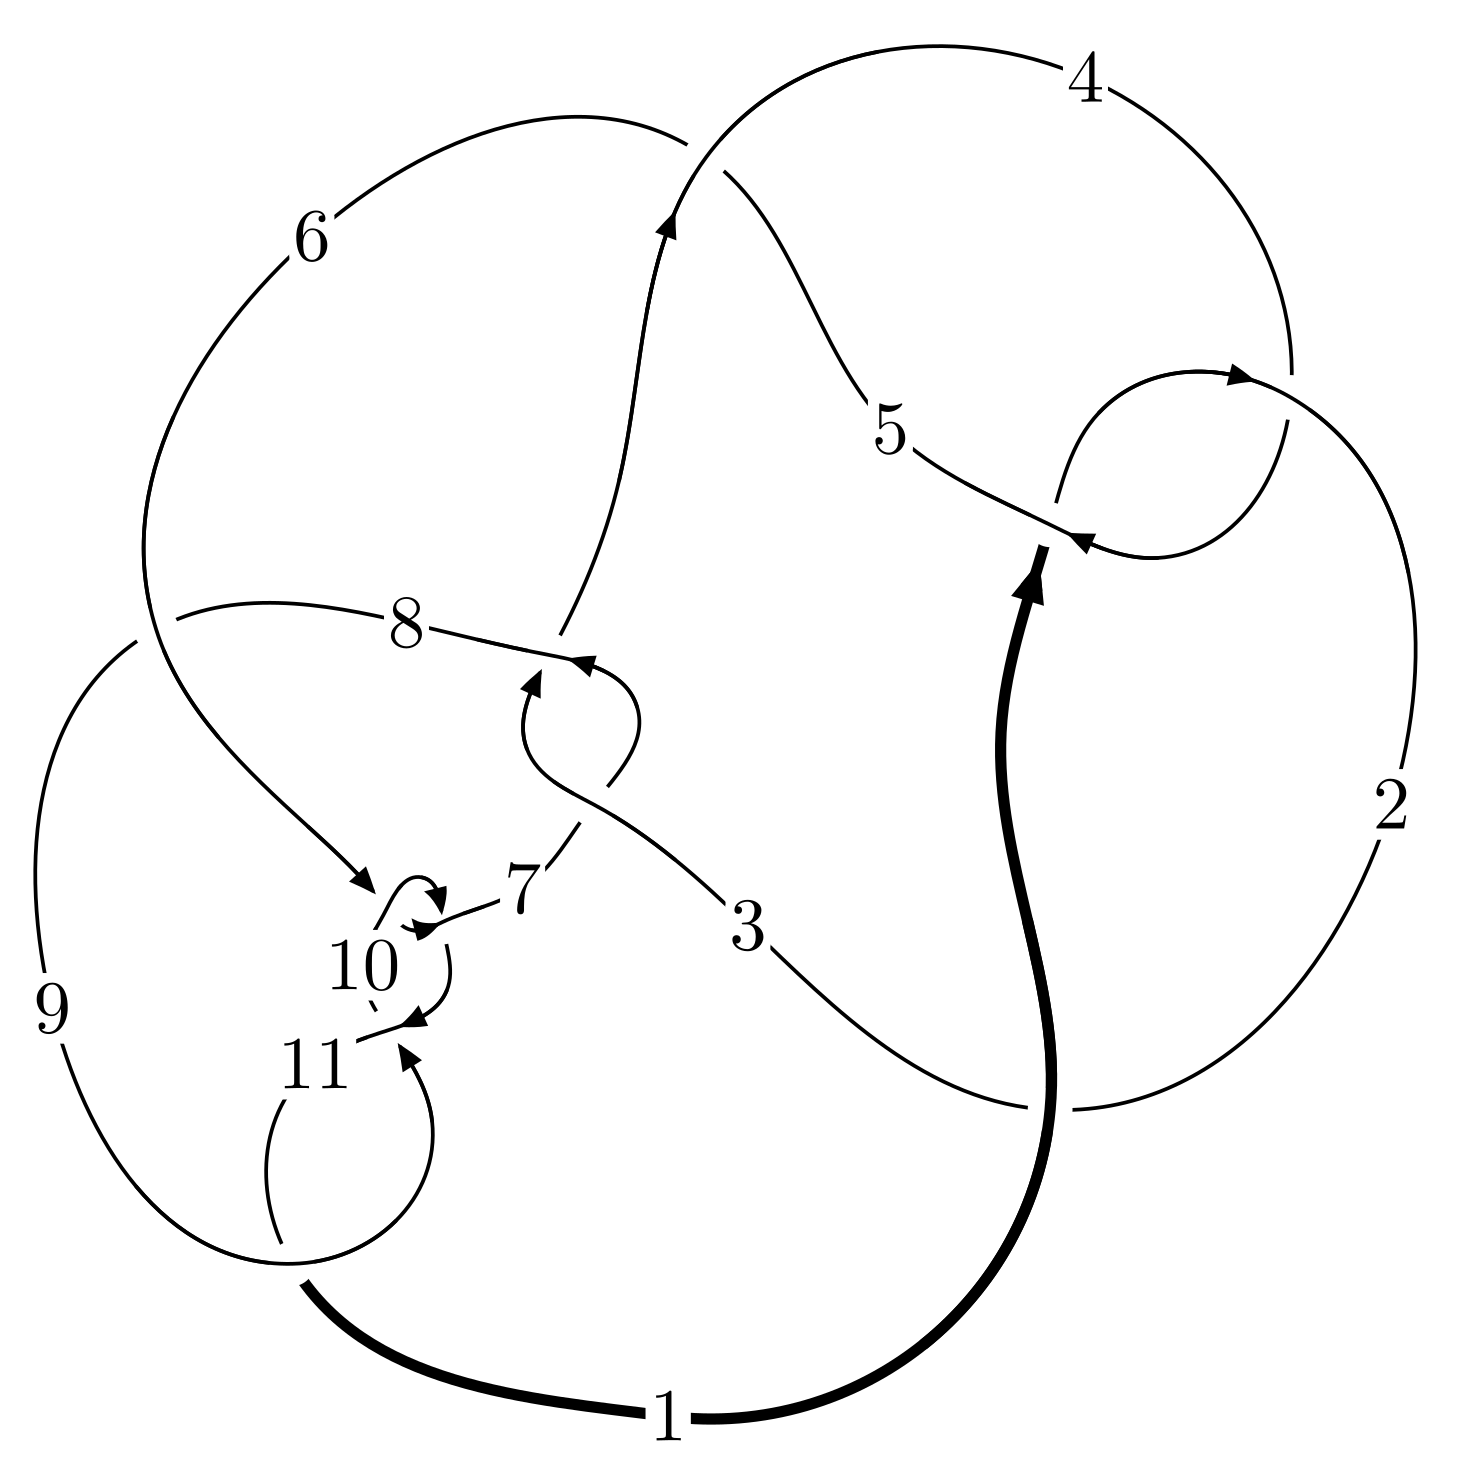
\includegraphics[width=112pt]{../../../GIT/diagram.site/Diagrams/png/297_11a_48.png}\\
\ \ \ A knot diagram\footnotemark}&
\allowdisplaybreaks
\textbf{Linearized knot diagam} \\
\cline{2-2}
 &
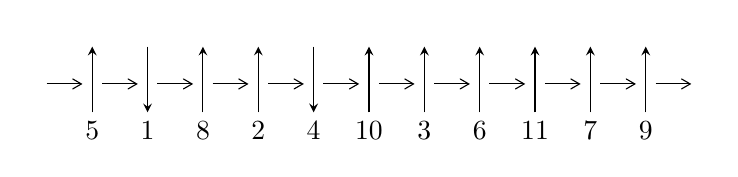
\begin{tikzpicture}[x=20pt, y=17pt]
	% nodes
	\node (C0) at (0, 0) {};
	\node (C1) at (1, 0) {};
	\node (C1U) at (1, +1) {};
	\node (C1D) at (1, -1) {5};

	\node (C2) at (2, 0) {};
	\node (C2U) at (2, +1) {};
	\node (C2D) at (2, -1) {1};

	\node (C3) at (3, 0) {};
	\node (C3U) at (3, +1) {};
	\node (C3D) at (3, -1) {8};

	\node (C4) at (4, 0) {};
	\node (C4U) at (4, +1) {};
	\node (C4D) at (4, -1) {2};

	\node (C5) at (5, 0) {};
	\node (C5U) at (5, +1) {};
	\node (C5D) at (5, -1) {4};

	\node (C6) at (6, 0) {};
	\node (C6U) at (6, +1) {};
	\node (C6D) at (6, -1) {10};

	\node (C7) at (7, 0) {};
	\node (C7U) at (7, +1) {};
	\node (C7D) at (7, -1) {3};

	\node (C8) at (8, 0) {};
	\node (C8U) at (8, +1) {};
	\node (C8D) at (8, -1) {6};

	\node (C9) at (9, 0) {};
	\node (C9U) at (9, +1) {};
	\node (C9D) at (9, -1) {11};

	\node (C10) at (10, 0) {};
	\node (C10U) at (10, +1) {};
	\node (C10D) at (10, -1) {7};

	\node (C11) at (11, 0) {};
	\node (C11U) at (11, +1) {};
	\node (C11D) at (11, -1) {9};
	\node (C12) at (12, 0) {};

	% arrows
	\draw[->,>={angle 60}]
	(C0) edge (C1) (C1) edge (C2) (C2) edge (C3) (C3) edge (C4) (C4) edge (C5) (C5) edge (C6) (C6) edge (C7) (C7) edge (C8) (C8) edge (C9) (C9) edge (C10) (C10) edge (C11) (C11) edge (C12) ;	\draw[->,>=stealth]
	(C1D) edge (C1U) (C2U) edge (C2D) (C3D) edge (C3U) (C4D) edge (C4U) (C5U) edge (C5D) (C6D) edge (C6U) (C7D) edge (C7U) (C8D) edge (C8U) (C9D) edge (C9U) (C10D) edge (C10U) (C11D) edge (C11U) ;
	\end{tikzpicture} \\
\hhline{~~} \\& 
\textbf{Solving Sequence} \\ \cline{2-2} 
 &
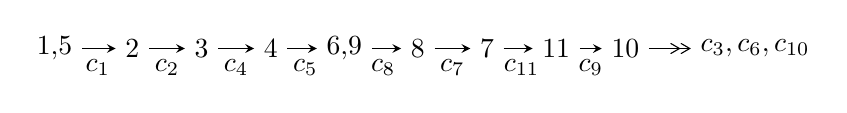
\begin{tikzpicture}[x=25pt, y=7pt]
	% node
	\node (A0) at (-1/8, 0) {1,5};
	\node (A1) at (1, 0) {2};
	\node (A2) at (2, 0) {3};
	\node (A3) at (3, 0) {4};
	\node (A4) at (65/16, 0) {6,9};
	\node (A5) at (41/8, 0) {8};
	\node (A6) at (49/8, 0) {7};
	\node (A7) at (57/8, 0) {11};
	\node (A8) at (65/8, 0) {10};
	\node (C1) at (1/2, -1) {$c_{1}$};
	\node (C2) at (3/2, -1) {$c_{2}$};
	\node (C3) at (5/2, -1) {$c_{4}$};
	\node (C4) at (7/2, -1) {$c_{5}$};
	\node (C5) at (37/8, -1) {$c_{8}$};
	\node (C6) at (45/8, -1) {$c_{7}$};
	\node (C7) at (53/8, -1) {$c_{11}$};
	\node (C8) at (61/8, -1) {$c_{9}$};
	\node (A9) at (10, 0) {$c_{3},c_{6},c_{10}$};

	% edge
	\draw[->,>=stealth]	
	(A0) edge (A1) (A1) edge (A2) (A2) edge (A3) (A3) edge (A4) (A4) edge (A5) (A5) edge (A6) (A6) edge (A7) (A7) edge (A8) ;
	\draw[->>,>={angle 60}]	
	(A8) edge (A9);
\end{tikzpicture} \\ 

\end{tabular} \\

\footnotetext{
The image of knot diagram is generated by the software ``\textbf{Draw programme}" developed by Andrew Bartholomew(\url{http://www.layer8.co.uk/maths/draw/index.htm\#Running-draw}), where we modified some parts for our purpose(\url{https://github.com/CATsTAILs/LinksPainter}).
}\phantom \\ \newline 
\centering \textbf{Ideals for irreducible components\footnotemark of $X_{\text{par}}$} 
 
\begin{align*}
I^u_{1}&=\langle 
-14 u^{61}+23 u^{60}+\cdots+4 b-7,\;-9 u^{61}+37 u^{60}+\cdots+4 a+12,\;u^{62}-4 u^{61}+\cdots+u+1\rangle \\
I^u_{2}&=\langle 
- a u+b- a,\;a^3+a^2 u-2 a u-2 a+1,\;u^2+u+1\rangle \\
\\
\end{align*}
\raggedright * 2 irreducible components of $\dim_{\mathbb{C}}=0$, with total 68 representations.\\
\footnotetext{All coefficients of polynomials are rational numbers. But the coefficients are sometimes approximated in decimal forms when there is not enough margin.}
\newpage
\renewcommand{\arraystretch}{1}
\centering \section*{I. $I^u_{1}= \langle -14 u^{61}+23 u^{60}+\cdots+4 b-7,\;-9 u^{61}+37 u^{60}+\cdots+4 a+12,\;u^{62}-4 u^{61}+\cdots+u+1 \rangle$}
\flushleft \textbf{(i) Arc colorings}\\
\begin{tabular}{m{7pt} m{180pt} m{7pt} m{180pt} }
\flushright $a_{1}=$&$\begin{pmatrix}1\\0\end{pmatrix}$ \\
\flushright $a_{5}=$&$\begin{pmatrix}0\\u\end{pmatrix}$ \\
\flushright $a_{2}=$&$\begin{pmatrix}1\\- u^2\end{pmatrix}$ \\
\flushright $a_{3}=$&$\begin{pmatrix}u^2+1\\- u^2\end{pmatrix}$ \\
\flushright $a_{4}=$&$\begin{pmatrix}- u\\u^3+u\end{pmatrix}$ \\
\flushright $a_{6}=$&$\begin{pmatrix}- u^3\\u^5+u^3+u\end{pmatrix}$ \\
\flushright $a_{9}=$&$\begin{pmatrix}\frac{9}{4} u^{61}-\frac{37}{4} u^{60}+\cdots-\frac{3}{4} u-3\\\frac{7}{2} u^{61}-\frac{23}{4} u^{60}+\cdots+\frac{13}{2} u+\frac{7}{4}\end{pmatrix}$ \\
\flushright $a_{8}=$&$\begin{pmatrix}\frac{11}{4} u^{61}-\frac{35}{2} u^{60}+\cdots-\frac{49}{4} u-\frac{35}{4}\\\frac{13}{2} u^{61}-\frac{47}{4} u^{60}+\cdots+\frac{23}{2} u+\frac{11}{4}\end{pmatrix}$ \\
\flushright $a_{7}=$&$\begin{pmatrix}\frac{13}{4} u^{61}-\frac{23}{2} u^{60}+\cdots-\frac{7}{4} u-\frac{13}{4}\\\frac{3}{2} u^{61}-\frac{1}{4} u^{60}+\cdots+\frac{13}{2} u+\frac{9}{4}\end{pmatrix}$ \\
\flushright $a_{11}=$&$\begin{pmatrix}-\frac{1}{4} u^{60}+\frac{3}{4} u^{59}+\cdots+\frac{5}{2} u+\frac{7}{4}\\\frac{1}{4} u^{61}- u^{60}+\cdots-\frac{5}{4} u-\frac{1}{4}\end{pmatrix}$ \\
\flushright $a_{10}=$&$\begin{pmatrix}-\frac{11}{4} u^{61}+\frac{47}{4} u^{60}+\cdots+\frac{7}{4} u+1\\-\frac{3}{4} u^{61}-\frac{1}{4} u^{60}+\cdots-\frac{17}{4} u-\frac{5}{2}\end{pmatrix}$\\ \flushright $a_{10}=$&$\begin{pmatrix}-\frac{11}{4} u^{61}+\frac{47}{4} u^{60}+\cdots+\frac{7}{4} u+1\\-\frac{3}{4} u^{61}-\frac{1}{4} u^{60}+\cdots-\frac{17}{4} u-\frac{5}{2}\end{pmatrix}$\\&\end{tabular}
\flushleft \textbf{(ii) Obstruction class $= -1$}\\~\\
\flushleft \textbf{(iii) Cusp Shapes $= 3 u^{61}+\frac{1}{2} u^{60}+\cdots+u+16$}\\~\\
\newpage\renewcommand{\arraystretch}{1}
\flushleft \textbf{(iv) u-Polynomials at the component}\newline \\
\begin{tabular}{m{50pt}|m{274pt}}
Crossings & \hspace{64pt}u-Polynomials at each crossing \\
\hline $$\begin{aligned}c_{1},c_{4}\end{aligned}$$&$\begin{aligned}
&u^{62}+4 u^{61}+\cdots- u+1
\end{aligned}$\\
\hline $$\begin{aligned}c_{2},c_{5}\end{aligned}$$&$\begin{aligned}
&u^{62}+20 u^{61}+\cdots-17 u+1
\end{aligned}$\\
\hline $$\begin{aligned}c_{3},c_{7}\end{aligned}$$&$\begin{aligned}
&u^{62}- u^{61}+\cdots+224 u-64
\end{aligned}$\\
\hline $$\begin{aligned}c_{6},c_{10}\end{aligned}$$&$\begin{aligned}
&u^{62}-3 u^{61}+\cdots+2 u-1
\end{aligned}$\\
\hline $$\begin{aligned}c_{8}\end{aligned}$$&$\begin{aligned}
&u^{62}+3 u^{61}+\cdots-4452 u-1201
\end{aligned}$\\
\hline $$\begin{aligned}c_{9},c_{11}\end{aligned}$$&$\begin{aligned}
&u^{62}-21 u^{61}+\cdots-16 u+1
\end{aligned}$\\
\hline
\end{tabular}\\~\\
\newpage\renewcommand{\arraystretch}{1}
\flushleft \textbf{(v) Riley Polynomials at the component}\newline \\
\begin{tabular}{m{50pt}|m{274pt}}
Crossings & \hspace{64pt}Riley Polynomials at each crossing \\
\hline $$\begin{aligned}c_{1},c_{4}\end{aligned}$$&$\begin{aligned}
&y^{62}+20 y^{61}+\cdots-17 y+1
\end{aligned}$\\
\hline $$\begin{aligned}c_{2},c_{5}\end{aligned}$$&$\begin{aligned}
&y^{62}+48 y^{61}+\cdots-369 y+1
\end{aligned}$\\
\hline $$\begin{aligned}c_{3},c_{7}\end{aligned}$$&$\begin{aligned}
&y^{62}-35 y^{61}+\cdots-37888 y+4096
\end{aligned}$\\
\hline $$\begin{aligned}c_{6},c_{10}\end{aligned}$$&$\begin{aligned}
&y^{62}-21 y^{61}+\cdots-16 y+1
\end{aligned}$\\
\hline $$\begin{aligned}c_{8}\end{aligned}$$&$\begin{aligned}
&y^{62}-17 y^{61}+\cdots-41957136 y+1442401
\end{aligned}$\\
\hline $$\begin{aligned}c_{9},c_{11}\end{aligned}$$&$\begin{aligned}
&y^{62}+43 y^{61}+\cdots-16 y+1
\end{aligned}$\\
\hline
\end{tabular}\\~\\
\newpage\flushleft \textbf{(vi) Complex Volumes and Cusp Shapes}
$$\begin{array}{c|c|c}  
\text{Solutions to }I^u_{1}& \I (\text{vol} + \sqrt{-1}CS) & \text{Cusp shape}\\
 \hline 
\begin{aligned}
u &= -0.580047 + 0.850451 I \\
a &= -0.615466 - 0.047953 I \\
b &= -0.105015 + 0.107324 I\end{aligned}
 & \phantom{-}0.46590 - 2.28716 I & \phantom{-}1.57514 + 4.44404 I \\ \hline\begin{aligned}
u &= -0.580047 - 0.850451 I \\
a &= -0.615466 + 0.047953 I \\
b &= -0.105015 - 0.107324 I\end{aligned}
 & \phantom{-}0.46590 + 2.28716 I & \phantom{-}1.57514 - 4.44404 I \\ \hline\begin{aligned}
u &= -0.708480 + 0.748571 I \\
a &= -0.625956 - 0.954656 I \\
b &= -0.035473 + 0.874104 I\end{aligned}
 & -0.06793 - 2.21961 I & \phantom{-}7.00000 + 3.72035 I \\ \hline\begin{aligned}
u &= -0.708480 - 0.748571 I \\
a &= -0.625956 + 0.954656 I \\
b &= -0.035473 - 0.874104 I\end{aligned}
 & -0.06793 + 2.21961 I & \phantom{-}7.00000 - 3.72035 I \\ \hline\begin{aligned}
u &= -0.176329 + 0.912969 I \\
a &= -0.631715 + 0.212995 I \\
b &= \phantom{-}0.204630 + 0.113298 I\end{aligned}
 & -1.47231 - 1.88154 I & \phantom{-}1.17198 + 4.94319 I \\ \hline\begin{aligned}
u &= -0.176329 - 0.912969 I \\
a &= -0.631715 - 0.212995 I \\
b &= \phantom{-}0.204630 - 0.113298 I\end{aligned}
 & -1.47231 + 1.88154 I & \phantom{-}1.17198 - 4.94319 I \\ \hline\begin{aligned}
u &= \phantom{-}0.067320 + 0.925637 I \\
a &= -1.65632 + 1.56093 I \\
b &= -0.021019 + 1.209610 I\end{aligned}
 & -5.17463 - 1.43170 I & -0.06499 + 2.83805 I \\ \hline\begin{aligned}
u &= \phantom{-}0.067320 - 0.925637 I \\
a &= -1.65632 - 1.56093 I \\
b &= -0.021019 - 1.209610 I\end{aligned}
 & -5.17463 + 1.43170 I & -0.06499 - 2.83805 I \\ \hline\begin{aligned}
u &= -0.762893 + 0.779001 I \\
a &= \phantom{-}0.88438 + 1.40384 I \\
b &= -0.547272 - 1.284430 I\end{aligned}
 & \phantom{-}0.86999 + 2.89738 I & \phantom{-0.000000 } 0 \\ \hline\begin{aligned}
u &= -0.762893 - 0.779001 I \\
a &= \phantom{-}0.88438 - 1.40384 I \\
b &= -0.547272 + 1.284430 I\end{aligned}
 & \phantom{-}0.86999 - 2.89738 I & \phantom{-0.000000 } 0\\
 \hline 
 \end{array}$$\newpage$$\begin{array}{c|c|c}  
\text{Solutions to }I^u_{1}& \I (\text{vol} + \sqrt{-1}CS) & \text{Cusp shape}\\
 \hline 
\begin{aligned}
u &= \phantom{-}0.672440 + 0.859246 I \\
a &= -1.094710 + 0.307283 I \\
b &= -0.15697 + 1.45420 I\end{aligned}
 & -1.87828 - 0.43024 I & \phantom{-0.000000 } 0 \\ \hline\begin{aligned}
u &= \phantom{-}0.672440 - 0.859246 I \\
a &= -1.094710 - 0.307283 I \\
b &= -0.15697 - 1.45420 I\end{aligned}
 & -1.87828 + 0.43024 I & \phantom{-0.000000 } 0 \\ \hline\begin{aligned}
u &= \phantom{-}0.113095 + 0.896419 I \\
a &= \phantom{-}1.43284 - 1.95950 I \\
b &= -0.35266 - 1.38822 I\end{aligned}
 & -4.68648 + 4.26236 I & \phantom{-}0.88079 - 2.61775 I \\ \hline\begin{aligned}
u &= \phantom{-}0.113095 - 0.896419 I \\
a &= \phantom{-}1.43284 + 1.95950 I \\
b &= -0.35266 + 1.38822 I\end{aligned}
 & -4.68648 - 4.26236 I & \phantom{-}0.88079 + 2.61775 I \\ \hline\begin{aligned}
u &= \phantom{-}0.848922 + 0.694333 I \\
a &= -0.858355 + 0.429131 I \\
b &= \phantom{-}0.287596 - 1.039470 I\end{aligned}
 & \phantom{-}3.14061 - 3.35098 I & \phantom{-0.000000 } 0 \\ \hline\begin{aligned}
u &= \phantom{-}0.848922 - 0.694333 I \\
a &= -0.858355 - 0.429131 I \\
b &= \phantom{-}0.287596 + 1.039470 I\end{aligned}
 & \phantom{-}3.14061 + 3.35098 I & \phantom{-0.000000 } 0 \\ \hline\begin{aligned}
u &= -0.288556 + 1.063810 I \\
a &= -0.278572 + 0.779132 I \\
b &= -0.996600 + 0.151978 I\end{aligned}
 & \phantom{-}1.97217 - 3.44390 I & \phantom{-0.000000 } 0 \\ \hline\begin{aligned}
u &= -0.288556 - 1.063810 I \\
a &= -0.278572 - 0.779132 I \\
b &= -0.996600 - 0.151978 I\end{aligned}
 & \phantom{-}1.97217 + 3.44390 I & \phantom{-0.000000 } 0 \\ \hline\begin{aligned}
u &= -0.172015 + 1.093990 I \\
a &= -1.05796 - 1.37125 I \\
b &= \phantom{-}0.117190 - 1.069160 I\end{aligned}
 & -3.80732 - 3.28559 I & \phantom{-0.000000 } 0 \\ \hline\begin{aligned}
u &= -0.172015 - 1.093990 I \\
a &= -1.05796 + 1.37125 I \\
b &= \phantom{-}0.117190 + 1.069160 I\end{aligned}
 & -3.80732 + 3.28559 I & \phantom{-0.000000 } 0\\
 \hline 
 \end{array}$$\newpage$$\begin{array}{c|c|c}  
\text{Solutions to }I^u_{1}& \I (\text{vol} + \sqrt{-1}CS) & \text{Cusp shape}\\
 \hline 
\begin{aligned}
u &= \phantom{-}0.872766 + 0.690242 I \\
a &= \phantom{-}0.873901 - 0.662198 I \\
b &= -0.58873 + 1.46893 I\end{aligned}
 & \phantom{-}4.38951 - 9.08805 I & \phantom{-0.000000 } 0 \\ \hline\begin{aligned}
u &= \phantom{-}0.872766 - 0.690242 I \\
a &= \phantom{-}0.873901 + 0.662198 I \\
b &= -0.58873 - 1.46893 I\end{aligned}
 & \phantom{-}4.38951 + 9.08805 I & \phantom{-0.000000 } 0 \\ \hline\begin{aligned}
u &= \phantom{-}0.673310 + 0.886698 I \\
a &= \phantom{-}0.848443 - 0.513970 I \\
b &= -0.08966 - 1.42530 I\end{aligned}
 & -1.96729 + 5.63314 I & \phantom{-0.000000 } 0 \\ \hline\begin{aligned}
u &= \phantom{-}0.673310 - 0.886698 I \\
a &= \phantom{-}0.848443 + 0.513970 I \\
b &= -0.08966 + 1.42530 I\end{aligned}
 & -1.96729 - 5.63314 I & \phantom{-0.000000 } 0 \\ \hline\begin{aligned}
u &= \phantom{-}0.811900 + 0.775479 I \\
a &= -1.206090 - 0.072648 I \\
b &= \phantom{-}0.416947 + 0.445355 I\end{aligned}
 & \phantom{-}4.85281 - 0.38708 I & \phantom{-0.000000 } 0 \\ \hline\begin{aligned}
u &= \phantom{-}0.811900 - 0.775479 I \\
a &= -1.206090 + 0.072648 I \\
b &= \phantom{-}0.416947 - 0.445355 I\end{aligned}
 & \phantom{-}4.85281 + 0.38708 I & \phantom{-0.000000 } 0 \\ \hline\begin{aligned}
u &= -0.193615 + 1.121270 I \\
a &= \phantom{-}0.76073 + 1.80584 I \\
b &= -0.50338 + 1.40284 I\end{aligned}
 & -2.88060 - 8.87825 I & \phantom{-0.000000 } 0 \\ \hline\begin{aligned}
u &= -0.193615 - 1.121270 I \\
a &= \phantom{-}0.76073 - 1.80584 I \\
b &= -0.50338 - 1.40284 I\end{aligned}
 & -2.88060 + 8.87825 I & \phantom{-0.000000 } 0 \\ \hline\begin{aligned}
u &= -0.491392 + 1.033550 I \\
a &= \phantom{-}0.487519 + 1.001310 I \\
b &= -0.126717 + 1.022770 I\end{aligned}
 & -1.94981 - 3.50251 I & \phantom{-0.000000 } 0 \\ \hline\begin{aligned}
u &= -0.491392 - 1.033550 I \\
a &= \phantom{-}0.487519 - 1.001310 I \\
b &= -0.126717 - 1.022770 I\end{aligned}
 & -1.94981 + 3.50251 I & \phantom{-0.000000 } 0\\
 \hline 
 \end{array}$$\newpage$$\begin{array}{c|c|c}  
\text{Solutions to }I^u_{1}& \I (\text{vol} + \sqrt{-1}CS) & \text{Cusp shape}\\
 \hline 
\begin{aligned}
u &= -0.740943 + 0.874063 I \\
a &= \phantom{-}1.87255 + 0.82263 I \\
b &= -1.074740 + 0.047853 I\end{aligned}
 & \phantom{-}4.66247 - 2.81474 I & \phantom{-0.000000 } 0 \\ \hline\begin{aligned}
u &= -0.740943 - 0.874063 I \\
a &= \phantom{-}1.87255 - 0.82263 I \\
b &= -1.074740 - 0.047853 I\end{aligned}
 & \phantom{-}4.66247 + 2.81474 I & \phantom{-0.000000 } 0 \\ \hline\begin{aligned}
u &= \phantom{-}0.866327 + 0.751351 I \\
a &= \phantom{-}1.39239 - 0.33135 I \\
b &= -1.227950 + 0.228420 I\end{aligned}
 & \phantom{-}9.59400 - 2.64881 I & \phantom{-0.000000 } 0 \\ \hline\begin{aligned}
u &= \phantom{-}0.866327 - 0.751351 I \\
a &= \phantom{-}1.39239 + 0.33135 I \\
b &= -1.227950 - 0.228420 I\end{aligned}
 & \phantom{-}9.59400 + 2.64881 I & \phantom{-0.000000 } 0 \\ \hline\begin{aligned}
u &= -0.446047 + 1.065130 I \\
a &= -0.990242 - 0.647003 I \\
b &= -0.466356 - 1.245930 I\end{aligned}
 & -1.36538 + 1.65817 I & \phantom{-0.000000 } 0 \\ \hline\begin{aligned}
u &= -0.446047 - 1.065130 I \\
a &= -0.990242 + 0.647003 I \\
b &= -0.466356 + 1.245930 I\end{aligned}
 & -1.36538 - 1.65817 I & \phantom{-0.000000 } 0 \\ \hline\begin{aligned}
u &= \phantom{-}0.838512 + 0.820293 I \\
a &= \phantom{-}1.45343 + 0.32563 I \\
b &= -0.784520 - 1.117280 I\end{aligned}
 & \phantom{-}6.92919 + 4.19000 I & \phantom{-0.000000 } 0 \\ \hline\begin{aligned}
u &= \phantom{-}0.838512 - 0.820293 I \\
a &= \phantom{-}1.45343 - 0.32563 I \\
b &= -0.784520 + 1.117280 I\end{aligned}
 & \phantom{-}6.92919 - 4.19000 I & \phantom{-0.000000 } 0 \\ \hline\begin{aligned}
u &= -0.696514 + 0.949067 I \\
a &= -2.10523 + 0.43360 I \\
b &= \phantom{-}0.084369 - 0.956151 I\end{aligned}
 & -0.66167 - 3.18112 I & \phantom{-0.000000 } 0 \\ \hline\begin{aligned}
u &= -0.696514 - 0.949067 I \\
a &= -2.10523 - 0.43360 I \\
b &= \phantom{-}0.084369 + 0.956151 I\end{aligned}
 & -0.66167 + 3.18112 I & \phantom{-0.000000 } 0\\
 \hline 
 \end{array}$$\newpage$$\begin{array}{c|c|c}  
\text{Solutions to }I^u_{1}& \I (\text{vol} + \sqrt{-1}CS) & \text{Cusp shape}\\
 \hline 
\begin{aligned}
u &= -0.728645 + 0.950887 I \\
a &= \phantom{-}2.59637 - 0.18053 I \\
b &= -0.54347 + 1.35036 I\end{aligned}
 & \phantom{-}0.34590 - 8.55449 I & \phantom{-0.000000 } 0 \\ \hline\begin{aligned}
u &= -0.728645 - 0.950887 I \\
a &= \phantom{-}2.59637 + 0.18053 I \\
b &= -0.54347 - 1.35036 I\end{aligned}
 & \phantom{-}0.34590 + 8.55449 I & \phantom{-0.000000 } 0 \\ \hline\begin{aligned}
u &= -0.760261 + 0.159745 I \\
a &= \phantom{-}0.938749 - 0.389340 I \\
b &= -0.56323 + 1.31677 I\end{aligned}
 & \phantom{-}1.40736 - 5.86221 I & \phantom{-}11.56645 + 5.83230 I \\ \hline\begin{aligned}
u &= -0.760261 - 0.159745 I \\
a &= \phantom{-}0.938749 + 0.389340 I \\
b &= -0.56323 - 1.31677 I\end{aligned}
 & \phantom{-}1.40736 + 5.86221 I & \phantom{-}11.56645 - 5.83230 I \\ \hline\begin{aligned}
u &= \phantom{-}0.752971 + 0.970116 I \\
a &= -0.630063 + 0.503155 I \\
b &= \phantom{-}0.456679 - 0.367835 I\end{aligned}
 & \phantom{-}4.25170 + 6.26267 I & \phantom{-0.000000 } 0 \\ \hline\begin{aligned}
u &= \phantom{-}0.752971 - 0.970116 I \\
a &= -0.630063 - 0.503155 I \\
b &= \phantom{-}0.456679 + 0.367835 I\end{aligned}
 & \phantom{-}4.25170 - 6.26267 I & \phantom{-0.000000 } 0 \\ \hline\begin{aligned}
u &= \phantom{-}0.789356 + 0.948317 I \\
a &= \phantom{-}0.026334 - 1.083390 I \\
b &= -0.815193 + 1.043280 I\end{aligned}
 & \phantom{-}6.52873 + 1.87763 I & \phantom{-0.000000 } 0 \\ \hline\begin{aligned}
u &= \phantom{-}0.789356 - 0.948317 I \\
a &= \phantom{-}0.026334 + 1.083390 I \\
b &= -0.815193 - 1.043280 I\end{aligned}
 & \phantom{-}6.52873 - 1.87763 I & \phantom{-0.000000 } 0 \\ \hline\begin{aligned}
u &= -0.744263\phantom{ +0.000000I} \\
a &= \phantom{-}1.16786\phantom{ +0.000000I} \\
b &= -1.09986\phantom{ +0.000000I}\end{aligned}
 & \phantom{-}5.44766\phantom{ +0.000000I} & \phantom{-}16.7720\phantom{ +0.000000I} \\ \hline\begin{aligned}
u &= \phantom{-}0.741510 + 1.026060 I \\
a &= -2.01086 + 0.29598 I \\
b &= \phantom{-}0.288482 + 1.092220 I\end{aligned}
 & \phantom{-}2.12433 + 9.28782 I & \phantom{-0.000000 } 0\\
 \hline 
 \end{array}$$\newpage$$\begin{array}{c|c|c}  
\text{Solutions to }I^u_{1}& \I (\text{vol} + \sqrt{-1}CS) & \text{Cusp shape}\\
 \hline 
\begin{aligned}
u &= \phantom{-}0.741510 - 1.026060 I \\
a &= -2.01086 - 0.29598 I \\
b &= \phantom{-}0.288482 - 1.092220 I\end{aligned}
 & \phantom{-}2.12433 - 9.28782 I & \phantom{-0.000000 } 0 \\ \hline\begin{aligned}
u &= \phantom{-}0.774379 + 1.004960 I \\
a &= \phantom{-}1.35473 - 1.13843 I \\
b &= -1.218840 - 0.287269 I\end{aligned}
 & \phantom{-}8.80808 + 8.74834 I & \phantom{-0.000000 } 0 \\ \hline\begin{aligned}
u &= \phantom{-}0.774379 - 1.004960 I \\
a &= \phantom{-}1.35473 + 1.13843 I \\
b &= -1.218840 + 0.287269 I\end{aligned}
 & \phantom{-}8.80808 - 8.74834 I & \phantom{-0.000000 } 0 \\ \hline\begin{aligned}
u &= \phantom{-}0.749728 + 1.037360 I \\
a &= \phantom{-}2.34145 - 0.53630 I \\
b &= -0.56778 - 1.49568 I\end{aligned}
 & \phantom{-}3.3199 + 15.1181 I & \phantom{-0.000000 } 0 \\ \hline\begin{aligned}
u &= \phantom{-}0.749728 - 1.037360 I \\
a &= \phantom{-}2.34145 + 0.53630 I \\
b &= -0.56778 + 1.49568 I\end{aligned}
 & \phantom{-}3.3199 - 15.1181 I & \phantom{-0.000000 } 0 \\ \hline\begin{aligned}
u &= -0.675568 + 0.188318 I \\
a &= -0.786334 + 0.175025 I \\
b &= \phantom{-}0.053146 - 0.874363 I\end{aligned}
 & \phantom{-}0.358267 - 0.639742 I & \phantom{-}9.73626 + 0.89260 I \\ \hline\begin{aligned}
u &= -0.675568 - 0.188318 I \\
a &= -0.786334 - 0.175025 I \\
b &= \phantom{-}0.053146 + 0.874363 I\end{aligned}
 & \phantom{-}0.358267 + 0.639742 I & \phantom{-}9.73626 - 0.89260 I \\ \hline\begin{aligned}
u &= -0.017068 + 0.625651 I \\
a &= \phantom{-}0.059805 - 1.358870 I \\
b &= -0.665979 - 0.287190 I\end{aligned}
 & \phantom{-}0.589690 + 0.350421 I & \phantom{-}8.57728 - 0.80469 I \\ \hline\begin{aligned}
u &= -0.017068 - 0.625651 I \\
a &= \phantom{-}0.059805 + 1.358870 I \\
b &= -0.665979 + 0.287190 I\end{aligned}
 & \phantom{-}0.589690 - 0.350421 I & \phantom{-}8.57728 + 0.80469 I \\ \hline\begin{aligned}
u &= \phantom{-}0.361194 + 0.064869 I \\
a &= -0.06161 - 2.33790 I \\
b &= -0.267132 + 1.196310 I\end{aligned}
 & -2.33982 - 2.66219 I & \phantom{-}4.81398 + 3.49490 I\\
 \hline 
 \end{array}$$\newpage$$\begin{array}{c|c|c}  
\text{Solutions to }I^u_{1}& \I (\text{vol} + \sqrt{-1}CS) & \text{Cusp shape}\\
 \hline 
\begin{aligned}
u &= \phantom{-}0.361194 - 0.064869 I \\
a &= -0.06161 + 2.33790 I \\
b &= -0.267132 - 1.196310 I\end{aligned}
 & -2.33982 + 2.66219 I & \phantom{-}4.81398 - 3.49490 I \\ \hline\begin{aligned}
u &= -0.246452\phantom{ +0.000000I} \\
a &= -1.59617\phantom{ +0.000000I} \\
b &= -0.280872\phantom{ +0.000000I}\end{aligned}
 & \phantom{-}0.790964\phantom{ +0.000000I} & \phantom{-}12.7580\phantom{ +0.000000I}\\
 \hline 
 \end{array}$$\newpage\newpage\renewcommand{\arraystretch}{1}
\centering \section*{II. $I^u_{2}= \langle - a u+b- a,\;a^3+a^2 u-2 a u-2 a+1,\;u^2+u+1 \rangle$}
\flushleft \textbf{(i) Arc colorings}\\
\begin{tabular}{m{7pt} m{180pt} m{7pt} m{180pt} }
\flushright $a_{1}=$&$\begin{pmatrix}1\\0\end{pmatrix}$ \\
\flushright $a_{5}=$&$\begin{pmatrix}0\\u\end{pmatrix}$ \\
\flushright $a_{2}=$&$\begin{pmatrix}1\\u+1\end{pmatrix}$ \\
\flushright $a_{3}=$&$\begin{pmatrix}- u\\u+1\end{pmatrix}$ \\
\flushright $a_{4}=$&$\begin{pmatrix}- u\\u+1\end{pmatrix}$ \\
\flushright $a_{6}=$&$\begin{pmatrix}-1\\0\end{pmatrix}$ \\
\flushright $a_{9}=$&$\begin{pmatrix}a\\a u+a\end{pmatrix}$ \\
\flushright $a_{8}=$&$\begin{pmatrix}- a u\\a u+a\end{pmatrix}$ \\
\flushright $a_{7}=$&$\begin{pmatrix}- a u\\a u+a\end{pmatrix}$ \\
\flushright $a_{11}=$&$\begin{pmatrix}a^2 u+a^2+1\\a^2 u\end{pmatrix}$ \\
\flushright $a_{10}=$&$\begin{pmatrix}a^2 u+a^2+a u- u\\a^2 u- a u- a+1\end{pmatrix}$\\ \flushright $a_{10}=$&$\begin{pmatrix}a^2 u+a^2+a u- u\\a^2 u- a u- a+1\end{pmatrix}$\\&\end{tabular}
\flushleft \textbf{(ii) Obstruction class $= 1$}\\~\\
\flushleft \textbf{(iii) Cusp Shapes $= 6 a^2 u+a^2-4 a u-5 a+u+14$}\\~\\
\newpage\renewcommand{\arraystretch}{1}
\flushleft \textbf{(iv) u-Polynomials at the component}\newline \\
\begin{tabular}{m{50pt}|m{274pt}}
Crossings & \hspace{64pt}u-Polynomials at each crossing \\
\hline $$\begin{aligned}c_{1},c_{2},c_{5}\end{aligned}$$&$\begin{aligned}
&(u^2+u+1)^3
\end{aligned}$\\
\hline $$\begin{aligned}c_{3},c_{7}\end{aligned}$$&$\begin{aligned}
&u^6
\end{aligned}$\\
\hline $$\begin{aligned}c_{4}\end{aligned}$$&$\begin{aligned}
&(u^2- u+1)^3
\end{aligned}$\\
\hline $$\begin{aligned}c_{6}\end{aligned}$$&$\begin{aligned}
&(u^3- u^2+1)^2
\end{aligned}$\\
\hline $$\begin{aligned}c_{8},c_{11}\end{aligned}$$&$\begin{aligned}
&(u^3- u^2+2 u-1)^2
\end{aligned}$\\
\hline $$\begin{aligned}c_{9}\end{aligned}$$&$\begin{aligned}
&(u^3+u^2+2 u+1)^2
\end{aligned}$\\
\hline $$\begin{aligned}c_{10}\end{aligned}$$&$\begin{aligned}
&(u^3+u^2-1)^2
\end{aligned}$\\
\hline
\end{tabular}\\~\\
\newpage\renewcommand{\arraystretch}{1}
\flushleft \textbf{(v) Riley Polynomials at the component}\newline \\
\begin{tabular}{m{50pt}|m{274pt}}
Crossings & \hspace{64pt}Riley Polynomials at each crossing \\
\hline $$\begin{aligned}c_{1},c_{2},c_{4}\\c_{5}\end{aligned}$$&$\begin{aligned}
&(y^2+y+1)^3
\end{aligned}$\\
\hline $$\begin{aligned}c_{3},c_{7}\end{aligned}$$&$\begin{aligned}
&y^6
\end{aligned}$\\
\hline $$\begin{aligned}c_{6},c_{10}\end{aligned}$$&$\begin{aligned}
&(y^3- y^2+2 y-1)^2
\end{aligned}$\\
\hline $$\begin{aligned}c_{8},c_{9},c_{11}\end{aligned}$$&$\begin{aligned}
&(y^3+3 y^2+2 y-1)^2
\end{aligned}$\\
\hline
\end{tabular}\\~\\
\newpage\flushleft \textbf{(vi) Complex Volumes and Cusp Shapes}
$$\begin{array}{c|c|c}  
\text{Solutions to }I^u_{2}& \I (\text{vol} + \sqrt{-1}CS) & \text{Cusp shape}\\
 \hline 
\begin{aligned}
u &= -0.500000 + 0.866025 I \\
a &= -1.024480 - 0.839835 I \\
b &= \phantom{-}0.215080 - 1.307140 I\end{aligned}
 & -3.02413 - 4.85801 I & \phantom{-}4.03424 + 5.28153 I \\ \hline\begin{aligned}
u &= -0.500000 + 0.866025 I \\
a &= \phantom{-}1.239560 + 0.467306 I \\
b &= \phantom{-}0.215080 + 1.307140 I\end{aligned}
 & -3.02413 + 0.79824 I & \phantom{-}2.74410 - 0.29766 I \\ \hline\begin{aligned}
u &= -0.500000 + 0.866025 I \\
a &= \phantom{-}0.284920 - 0.493496 I \\
b &= \phantom{-}0.569840\phantom{ +0.000000I}\end{aligned}
 & \phantom{-}1.11345 - 2.02988 I & \phantom{-}12.72167 + 1.07831 I \\ \hline\begin{aligned}
u &= -0.500000 - 0.866025 I \\
a &= -1.024480 + 0.839835 I \\
b &= \phantom{-}0.215080 + 1.307140 I\end{aligned}
 & -3.02413 + 4.85801 I & \phantom{-}4.03424 - 5.28153 I \\ \hline\begin{aligned}
u &= -0.500000 - 0.866025 I \\
a &= \phantom{-}1.239560 - 0.467306 I \\
b &= \phantom{-}0.215080 - 1.307140 I\end{aligned}
 & -3.02413 - 0.79824 I & \phantom{-}2.74410 + 0.29766 I \\ \hline\begin{aligned}
u &= -0.500000 - 0.866025 I \\
a &= \phantom{-}0.284920 + 0.493496 I \\
b &= \phantom{-}0.569840\phantom{ +0.000000I}\end{aligned}
 & \phantom{-}1.11345 + 2.02988 I & \phantom{-}12.72167 - 1.07831 I\\
 \hline 
 \end{array}$$\newpage
\newpage\renewcommand{\arraystretch}{1}
\centering \section*{ III. u-Polynomials}
\begin{tabular}{m{50pt}|m{274pt}}
Crossings & \hspace{64pt}u-Polynomials at each crossing \\
\hline $$\begin{aligned}c_{1}\end{aligned}$$&$\begin{aligned}
&((u^2+u+1)^3)(u^{62}+4 u^{61}+\cdots- u+1)
\end{aligned}$\\
\hline $$\begin{aligned}c_{2},c_{5}\end{aligned}$$&$\begin{aligned}
&((u^2+u+1)^3)(u^{62}+20 u^{61}+\cdots-17 u+1)
\end{aligned}$\\
\hline $$\begin{aligned}c_{3},c_{7}\end{aligned}$$&$\begin{aligned}
&u^6(u^{62}- u^{61}+\cdots+224 u-64)
\end{aligned}$\\
\hline $$\begin{aligned}c_{4}\end{aligned}$$&$\begin{aligned}
&((u^2- u+1)^3)(u^{62}+4 u^{61}+\cdots- u+1)
\end{aligned}$\\
\hline $$\begin{aligned}c_{6}\end{aligned}$$&$\begin{aligned}
&((u^3- u^2+1)^2)(u^{62}-3 u^{61}+\cdots+2 u-1)
\end{aligned}$\\
\hline $$\begin{aligned}c_{8}\end{aligned}$$&$\begin{aligned}
&((u^3- u^2+2 u-1)^2)(u^{62}+3 u^{61}+\cdots-4452 u-1201)
\end{aligned}$\\
\hline $$\begin{aligned}c_{9}\end{aligned}$$&$\begin{aligned}
&((u^3+u^2+2 u+1)^2)(u^{62}-21 u^{61}+\cdots-16 u+1)
\end{aligned}$\\
\hline $$\begin{aligned}c_{10}\end{aligned}$$&$\begin{aligned}
&((u^3+u^2-1)^2)(u^{62}-3 u^{61}+\cdots+2 u-1)
\end{aligned}$\\
\hline $$\begin{aligned}c_{11}\end{aligned}$$&$\begin{aligned}
&((u^3- u^2+2 u-1)^2)(u^{62}-21 u^{61}+\cdots-16 u+1)
\end{aligned}$\\
\hline
\end{tabular}\newpage\renewcommand{\arraystretch}{1}
\centering \section*{ IV. Riley Polynomials}
\begin{tabular}{m{50pt}|m{274pt}}
Crossings & \hspace{64pt}Riley Polynomials at each crossing \\
\hline $$\begin{aligned}c_{1},c_{4}\end{aligned}$$&$\begin{aligned}
&((y^2+y+1)^3)(y^{62}+20 y^{61}+\cdots-17 y+1)
\end{aligned}$\\
\hline $$\begin{aligned}c_{2},c_{5}\end{aligned}$$&$\begin{aligned}
&((y^2+y+1)^3)(y^{62}+48 y^{61}+\cdots-369 y+1)
\end{aligned}$\\
\hline $$\begin{aligned}c_{3},c_{7}\end{aligned}$$&$\begin{aligned}
&y^6(y^{62}-35 y^{61}+\cdots-37888 y+4096)
\end{aligned}$\\
\hline $$\begin{aligned}c_{6},c_{10}\end{aligned}$$&$\begin{aligned}
&((y^3- y^2+2 y-1)^2)(y^{62}-21 y^{61}+\cdots-16 y+1)
\end{aligned}$\\
\hline $$\begin{aligned}c_{8}\end{aligned}$$&$\begin{aligned}
&((y^3+3 y^2+2 y-1)^2)(y^{62}-17 y^{61}+\cdots-4.19571\times10^{7} y+1442401)
\end{aligned}$\\
\hline $$\begin{aligned}c_{9},c_{11}\end{aligned}$$&$\begin{aligned}
&((y^3+3 y^2+2 y-1)^2)(y^{62}+43 y^{61}+\cdots-16 y+1)
\end{aligned}$\\
\hline
\end{tabular}
\vskip 2pc
\end{document}